% !TEX program = xelatex

\documentclass{resume}
\usepackage{graphicx}
\usepackage{tabu}
\usepackage{multirow}
% \usepackage{progressbar}
\usepackage{hyperref}
% \usepackage{zh_CN-Adobefonts_external} % Simplified Chinese Support using external fonts (./fonts/zh_CN-Adobe/)
% \usepackage{zh_CN-Adobefonts_internal} % Simplified Chinese Support using system fonts

\begin{document}
\pagenumbering{gobble} % suppress displaying page number

\noindent\begin{minipage}{0.3\textwidth}
  % adapt widths of minipages to your needs
  % change Large font here
  \Large{
    \textbf{Gen LI}\\
    % & {Python~}\progressbar{0.75}
    \email{rami3l@foxmail.com}   \\
    \phone{+33 (0)7 49 99 05 67} \\
    % & \linkedin[billryan8]{https://www.linkedin.com/in/billryan8} \\
    \github[github.com/rami3l]{https://github.com/rami3l}
  }
\end{minipage}
\hfill%
\begin{minipage}{0.6\textwidth}\raggedleft
  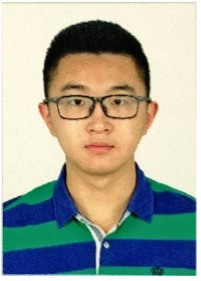
\includegraphics[width=0.88in]{avatar}
\end{minipage}

\section{Formation}
\datedsubsection{\textbf{École Centrale de Nantes (ECN)} Nantes, France}{Depuis Sept. 2020}
\textit{Cycle Ingénieur} (Informatique) : Programme double diplôme avec Centrale Pékin

\datedsubsection{\textbf{Université de Beihang (BUAA) - École Centrale Pékin} Pékin, Chine}{Sept. 2017 - Juin 2020}
2ème \& 3ème année : Étude des sciences en français (GPA : 3.6647)
\begin{itemize}
  \item Mathématiques, Physique, Science Industrielle, Programmation, …
\end{itemize}
1ère année : Étude intensive de la langue française (générale \& scientifique)


\section{Expérience Professionnelle}
\datedsubsection{\textbf{BUAA} - \href{https://github.com/BUAA-SE-Compiling/rurikawa}{\textit{Rurikawa} : Évaluation des Travaux Pratiques Informatiques}}{Depuis Juin 2020}
\role{Rust, Docker (via Bollard)}{Projet en équipe}
Système de style \textit{Online Judge} automatisant l'évaluation des TP informatiques
\begin{itemize}
  \item Conception \& réalisation du sous-système d'exécution de code
  \item Contribution à la bibliothèque en amont (\textit{Bollard}, binding de Docker API en Rust)
\end{itemize}

\datedsubsection{\textbf{Projet Personel} - \href{https://github.com/rami3l/pacaptr}{\textit{Pacaptr} : Outil Multiplateforme de Gestion de Paquets}}{Depuis Juin 2020}
\role{Rust, Clap (bibliothèque Rust d'analyse d'arguments CLI)}{}
Emballage des gestionnaires de paquets dans la syntaxe de \textit{pacman} de \textit{Arch Linux}
\begin{itemize}
  \item Analyse des besoins, réalisation du projet, maintenance continue \& marketing
  \item Utilisation de CI/CD pour la détection des régressions et la distribution des paquets
  \item Contribution à la bibliothèque en amont (\textit{Clap})
\end{itemize}

\datedsubsection{\textbf{xxx Projects}}{Jan. 2015 -- Present}
\role{C, Python, Django, Linux}{Individual Projects, collaborated with xxx}
Brief introduction: xxx
\begin{itemize}
  \item Implemented xxx feature
  \item Optimized xxx 5\%
  \item xxx
\end{itemize}

\datedsubsection{\textbf{\LaTeX\ résumé template}}{May. 2015 -- Present}
\role{\LaTeX, Maintainer}{Individual Projects}
An elegant \LaTeX\ résumé template, https://github.com/billryan/resume
\begin{itemize}
  \item Easy to be further customized or extended
  \item Full support for unicode characters (e.g. CJK) with \XeLaTeX\
  \item FontAwesome 4.5.0 support
\end{itemize}

% Reference Test
%\datedsubsection{\textbf{Paper Title\cite{zaharia2012resilient}}}{May. 2015}
%An xxx optimized for xxx\cite{verma2015large}
%\begin{itemize}
%  \item main contribution
%\end{itemize}

% \section{\faCogs\ Skills}
% \begin{itemize}[parsep=0.5ex]
%   \item Programming Languages: C == Python > C++ > Java
%   \item Platform: Linux
%   \item Development: Web, xxx
% \end{itemize}

% \section{\faHeartO\ Honors and Awards}
% \datedline{\textit{\nth{1} Prize}, Award on xxx }{Jun. 2013}
% \datedline{Other awards}{2015}

\section{Miscellaneous}
\begin{itemize}[parsep=0.5ex]
  \item Blog: http://your.blog.me
  \item GitHub: https://github.com/username
  \item Languages: English - Fluent, Mandarin - Native speaker
\end{itemize}

%% Reference
%\newpage
%\bibliographystyle{IEEETran}
%\bibliography{mycite}
\end{document}
